\documentclass{article}
\textheight 23.5cm \textwidth 15.8cm
%\leftskip -1cm
\topmargin -1.5cm \oddsidemargin 0.3cm \evensidemargin -0.3cm
%\documentclass[final]{siamltex}

\usepackage{graphicx}
\usepackage{epsfig}
\usepackage{amsmath}
\usepackage{amsthm}
\usepackage{amssymb}
\usepackage{mathrsfs}
\usepackage{float}
\usepackage{multirow}
\usepackage{verbatim}
\usepackage{fancyhdr}
\usepackage{subfigure}
\usepackage{color}
\usepackage{mathtools}
\usepackage{mathrsfs}
%\usepackage{natbib}
\usepackage{sectsty}
%\usepackage[title]{appendix}
\usepackage{threeparttable}
\usepackage{dcolumn}
\usepackage{booktabs}
\usepackage{indentfirst}
\usepackage{setspace}
\usepackage{bm}
\usepackage{enumerate}
\usepackage{geometry}
\usepackage{ctex}

\title{计算方法第一次程序作业报告}
\author{PB19071405 王昊元}
\date{2022 年 04 月 06 日}

\begin{document}
\maketitle

\section{问题描述}

$I(\ln x) = \int_{1}^{2}\ln x\, dx$,取$\epsilon = 10^{-4}$,\ $h = 1$,试用Romberg公式计算积分直到

$$|R_{k, k} - R_{k - 1, k - 1}| < \epsilon$$

时停止,并做出 Romberg积分数值表。

\section{数值计算方法}

Romberg积分公式主要使用了\emph{外推算法},外推算法在不增加计算量的前提下提高了误差的精度。

算法中$j = 1$时,$R_{k, j}$即表示梯形积分,从梯形积分利用外推算法得到Simpson积分公式,

$$I(f) \approx T_{2n}(f) + \frac{1}{3}(T_{2n}(f) - T_n(f)) = \frac{4}{3}T_{2n} - \frac{1}{3}T_n = S_n$$

也就是算法中$j = 2$的情形,截断误差也从梯形积分的$O(h^2)$提高到了$O(h^4)$。
对$S_{2n}(f)$,$S_n(f)$再作一次线性组合则可以得到

$$I(f) \approx S_{2n}(f) + \frac{1}{15}(S_{2n}(f) - S_n(f)) = C_n(f)$$

我们利用外推算法通过Simpson积分得到了Cotes积分,对应算法$j = 3$的情况,
截断误差也提高到了$O(h^6)$。

根据上述推导过程及经验,我们可以得到Romberg计算公式:

$$R_{k, j} = R_{k, j - 1} + \frac{R_{k, j-1} - R_{k-1, j-1}}{4^{j-1} - 1},\quad k=2,3,\cdots$$

\section{结果}

实验结果截图如下:

\begin{figure}[H]
    \centering
    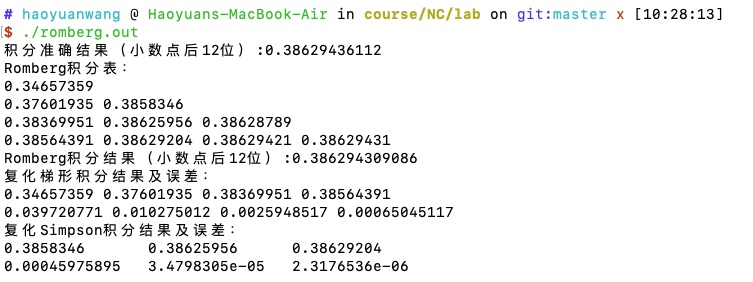
\includegraphics[width=0.7\textwidth]{./figs/lab1_result.jpg}
    \caption{程序运行结果}
    \label{program result}
\end{figure}

实验结果具体如下:

\text{Romberg}积分结果:$0.38629431$。

\begin{table}[H]
    \centering
    \caption{Romberg积分表}
    \begin{tabular}{cccc}
        \hline
        0.34657359 & ~ & ~ & ~ \\
        0.37601935 & 0.3858346 & ~ & ~ \\
        0.38369951 & 0.38625956 & 0.38628789 & ~ \\
        0.38564391 & 0.38629204 & 0.38629421 & 0.38629431 \\
        \hline
    \end{tabular}
\end{table}

\begin{table}[H]
    \centering
    \caption{复化梯形积分误差精度表}
    \begin{tabular}{|c|c|c|c|c|}
        \hline
        N & 1 & 2 & 4 & 8 \\
        \hline
        error & 0.039720771 & 0.010275012 & 0.0025948517 & 0.00065045117 \\
        \hline
        order & ~ & 1.9508 & 1.9854 & 1.9961 \\
        \hline
    \end{tabular}
\end{table}

\begin{table}[H]
    \centering
    \caption{复化Simpson积分误差精度表}
    \begin{tabular}{|c|c|c|c|c|}
        \hline
        N & 1 & 2 & 4 & 8 \\
        \hline
        error & ~ & 0.00045975895 & 3.4798305e-05 & 2.3176536e-06 \\
        \hline
        order & ~ & ~ & 3.7238 & 3.9083 \\
        \hline
    \end{tabular}
\end{table}

\section{结论}

比较积分的准确结果和Romberg积分的结果,可以发现误差提高到了$O(10^{-8})$,
而结束时$k$的值为4,这也验证了Romberg积分公式的正确性。

而从误差精度表中也可以发现,复化梯形积分和复化Simpson积分的误差分别为$O(10^{-2})$和$O(10^{-4})$,
符合我们的预期。

对于积分结果的每一列(即复化梯形积分、复化Simpson积分),可以看到随着N的逐渐增大,误差逐渐减小,
order也逐渐减小,也不断接近于$-2$与$-4$。
这也意味着在进行复化梯形积分和复化Simpson积分时,所取分点逐渐增多时,积分产生的截断误差也就越小。

\end{document}
